\renewcommand{\thepage}{}
\chapter{Realization}
\thispagestyle{empty}
\pagestyle{fancy}
\lhead{\small \bf  Chapitre 5: Realization}
\rhead{}
\chead{}
\renewcommand\thepage{\arabic{page}}
 \setcounter{minitocdepth}{1}
\minitoc
\clearpage
\section{Introduction}
\lettrine[lines=2,lhang=0.44,lraise=0,loversize=0.08,findent=-0.11em,slope=0.6em]%
{T}{} he $ IG� $ application is Web oriented. The analysis of the initial specifications has lead us to distinguish three different layers: 
\begin{itemize}
\item The UI interface allowing users to interact with the application (selecting objects and nodes, displaying graphs, etc.)
\item The logic that explores and organizes the data.
\item The data layer that contains the information specifying objects and entities.
\end{itemize}
\paragraph*{}
It is therefore obvious to adopt a 3-tiers architecture to implement the application: the presentation tier (the UI), the business tier (the logic layer) and the data layer. The implementation of the application was also based on the Model-View-Controller (MVC) [W12] paradigm. Using WEB 2.0 and MVC easily fit with the 3-tiers architecture and the needs expressed by Stradefi SA.
\section{The MVC Architecture}
\paragraph*{}
MVC [7][W12] - Model-View-Controller - is a design pattern for the architecture of Web applications.
\begin{figure}[h]
\centering
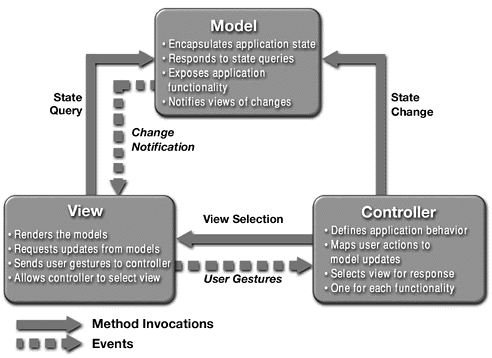
\includegraphics[scale=0.8]{mvc.png}
\caption{MVC model}
\end{figure}
\paragraph*{}
It is a widely adopted pattern, across many languages and implementation frameworks, whose purpose is to achieve a clean separation between three components of most any Web application:
\begin{itemize}
\item Model: business logic & processing
\item View: user interface (UI)
\item Controller: navigation & input
\end{itemize}
\paragraph*{}
MVC benefits fall into multiple categories:
\begin{itemize}
\item Separation of concerns in the codebase
\item Developer specialization and focus
\item Parallel development by separate teams
\end{itemize}
\paragraph*{}
In looking at these in a little more detail, it will become clear that the second two bullet-points are corollaries of the first.
\section{The 3-tiers architecture point of view of the $ IG� $}
\paragraph*{}
The development was based on HTML5, CSS3 and JavaScript. The presentation layer is based on these languages and technologies. The JIT library (�II.2.1), developed in JavaScript, combined with HTML allowed implementing easily the UI.
\paragraph*{}
The data layer, in the current state of the development uses only JSON files, however the application is open enough to support XML (using a DOM parser) or any other of structured data format (databases for instance).
\paragraph*{}
At the present time there's no clear separation between the business layer and the presentation layer. Indeed, we use the JIT native parser to parse JSON files and to render the corresponding radial graphs. As mentioned in the perspectives (� FUTUR), a very important part of the logic is not yet implemented and needs extra developments that do not depend on the JIT library.
\section{The MVC architecture point of view of the $IG�$}
\paragraph*{}
The model represents the underlying logical structure of the data used by the application (JSON files). This data model doesn't contain any information about the user interface and could therefore be used with other views and/or controllers.
\paragraph*{}
The view is the user interface itself. The view depends on the used device and adapts to the hardware constraints. The view cannot be reused except with compatible devices.
\paragraph*{}
The controller represents the way to communicate between the data model and the view. In the $IG�$ application two controllers have been taken into account: the first one allows the usage of a keyboard and mouse and the second one, which is suitable for mobile devices, allows the usage of the touch-pad and touch-screen.
\section{The logical architecture}
\paragraph*{}
The software components used by the application have been identified through the whole process of analysis and specification that has been conducted before the beginning of the development. The Web nature of the applications imposes the usage of an application server. The visualization of the radial graphs requires the usage of a rendering engine. despite the structured nature of the data used by the application, we made the choice not to consider a data base but rather use text files (JSON) that are natively supported by JavaScript. The overall logical architecture of the $IG�$ application is presented in the figure V.2.
\begin{figure}[h]
\centering
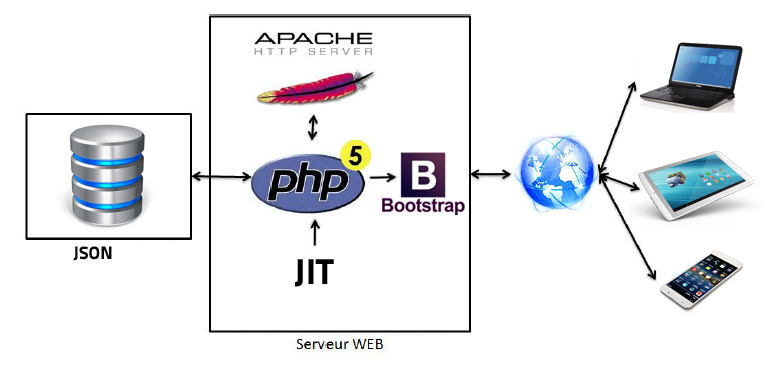
\includegraphics[scale=0.5, frame]{architechturesysteme.png}
\caption{Logical architecture}
\end{figure}
\paragraph*{}
The rendering engine is the JIT library (�II.2.1). The other software modules used for the development and the deployment of the application are: Apache HTTP server, PHP and Bootstrap.
\begin{itemize}
\item \textbf{Bootstrap:} Bootstrap[W13] is a free collection of tools for creating websites and web applications. It contains HTML and CSS-based design templates for typography, forms, buttons, navigation and other interface components, as well as optional JavaScript extensions. It is the No.1 project on GitHub with 65,000+ stars and 23,800 forks (as of March 2014) and has been used by NASA and MSNBC, among many others.
\item \textbf{PHP5:}PHP [W14] is a server-side scripting language designed for Web development but also used as a general-purpose programming language. As of January 2013, PHP was installed on more than 240 million websites (39\% of those sampled) and 2.1 million Web servers. Originally created by Rasmus Lerdorf in 1995, the reference implementation of PHP is now produced by The PHP Group. While PHP originally stood for Personal Home Page, it now stands for PHP: Hypertext Preprocessor, a recursive backronym.
PHP code can be simply mixed with HTML code, or it can be used in combination with various templating engines and Web frameworks. PHP code is usually processed by a PHP interpreter, which is usually implemented as a Web server's native module or a Common Gateway Interface (CGI) executable. After the PHP code is interpreted and executed, the Web server sends resulting output to its client in form of a generated Web page. PHP has also evolved to include a command-line interface (CLI) capability and can be used in standalone graphical applications.
PHP is free software released under the PHP License. PHP has been widely ported and can be deployed on most Web servers on almost every operating system and platform, free of charge.
\item \textbf{Apache HTTP Server} is a Web server application, it's a HTTP server created and maintained whitin the Apache foundation {\color[rgb]{0.41,0.41,0.41}\href{httpd.apache.org}{\textbf{10}}}. It's the most HTTP server popular on the World Wide Web {\color[rgb]{0.41,0.41,0.41}\href{http://webfoundation.org/}{\textbf{11}}}.
\end{itemize}
The Data layer is represented by various \textbf{Json}{\color[rgb]{0.41,0.41,0.41}\href{http://www.json.org/}{\textbf{8}}} files. 
\section{Class diagram}
\paragraph*{}
The design of the $IG�$ application provided us with the following class diagram (Figure V.3). Although the resulting implementation of $IG�$ is not object oriented, the class diagram helped us organizing the data layer, especially the structure of JSON files. We also used the OOTB features of JIT to implement the user interface.
\newpage
\begin{figure}[h]
\begin{center}
\includegraphics[scale=0.6, frame]{ClassDiagram.png}
\end{center}
\caption{$IG�$ Class Diagram}
\end{figure} 
\section{The sprints' achievement}
\paragraph*{}
Among all the requirements that have been defined in the $ IG� $ specifications, the most significant ones have been considered and defined as the product backlog. All of the considered requirements have been prioritized and organized as sprints. Actually four sprints has been achieved: "the project initiation sprints" (aka sprint "zero"), "the graph rendering sprint" (aka sprint "one"), "updating nodes' properties and managing relations sprint" (aka sprint "two") and the "localization sprint" (aka sprint "three").
\subsection{Sprint "zero": Project initiation}
\paragraph*{}
The project started by the analysis of the specifications given by Stradefi SA. Some conference calls have been done with Stradefi SA Office at Geneva to define the different roles of the team members and to identify the product backlog. A kick off meeting has also been done and officially started the project. The project plan was achieved in this sprint.
\begin{table}[h]
\begin{center}
\begin{tabular}{|p{7cm}|p{3cm}|p{3cm}|}
\hline
\multicolumn{3}{|c|}{Sprint "zero": Project initiation}  \\
\hline
\textbf{Tasks} & \textbf{Deadline} & \textbf{Date }\\
\hline
Kick-off meeting& 2 hours &  9 March \\
\hline
Server configuration & 3 Hours & 9 March \\
\hline
Architecture and methodology approval & 1 day & 9 March \\
\hline
\end{tabular}
\end{center}
\caption{Backlog product - Sprint "zero"}
\label{Backlog product - Sprint "zero"}
\end{table}
\subsection{Sprint "one": Rendering a radial graph}
\paragraph*{}
The development has really started during this sprint. We first focused on the parsing of JSON files, the identification of what could be represented as a node and what will play the role of a relation. Finally, the data extracted from the JSON files is given to the rendering engine in order to deal with it and to display the radial graph. The following table presents the sprint "one" backlog.
\begin{table}[h]
\begin{center}
\begin{tabular}{|p{7cm}|p{3cm}|p{3cm}|}
\hline
\multicolumn{3}{|c|}{Sprint "one": Rendering a radial graph}  \\
\hline
\textbf{Tasks} & \textbf{Deadline} & \textbf{Date }\\
\hline
Parsing of JSON file & 3 hours week & \multirow{7}{*}{27 March}  \\
\hline
Listing of the available objects & 4 hours & 27 March \\
\hline
Rendering the Radial Graph of the selected object & 3 hours & 27 March   \\
\hline
Managing the orientation (direction) of the relationships between nodes & 1 day & 27 March\\
\hline
Implementation of the mouseover event to display a summary of the information related to a given node & 3 hours & 27 March \\
\hline
Accessing to a node attributes and properties & 1 day & 27 March \\
\hline
Selection of the node of interest & 1 day & 27 March \\
\hline
\end{tabular}
\end{center}
\caption{Backlog product - Sprint "one"}
\label{Backlog product - Sprint "one"}
\end{table}
\subsubsection{Detailed design of Sprint "one"}
\paragraph*{}
The Figure V.4 presents the detailed design of sprint "one", its design the actions and events released, the user can use it to navigate on the application. 
\newpage
\begin{figure}[h]
\centering
\includegraphics[scale=0.7, frame]{renderingDiagram.png}
\caption{Rendering a radial graph Sequence Diagram}
\end{figure}
\subsubsection{Implementation and execution of Sprint "one"}
\paragraph*{}
When the user logs in, the first screen of the user interface the list of available objects, that he can access to (Figure V.5). The user can select an object in order to display the corresponding graph. 
\newpage
\begin{figure}[h]
\begin{center}
\includegraphics[scale=0.6, frame]{visualizeGraph.png}
\end{center}
\caption{The list of available objects}
\end{figure}
\paragraph*{}
When the user selects an object, the corresponding radial graph is displayed. The node corresponding to the object first selected by the user becomes the node of interest (Figure V.6).
\begin{figure}[h]
\centering
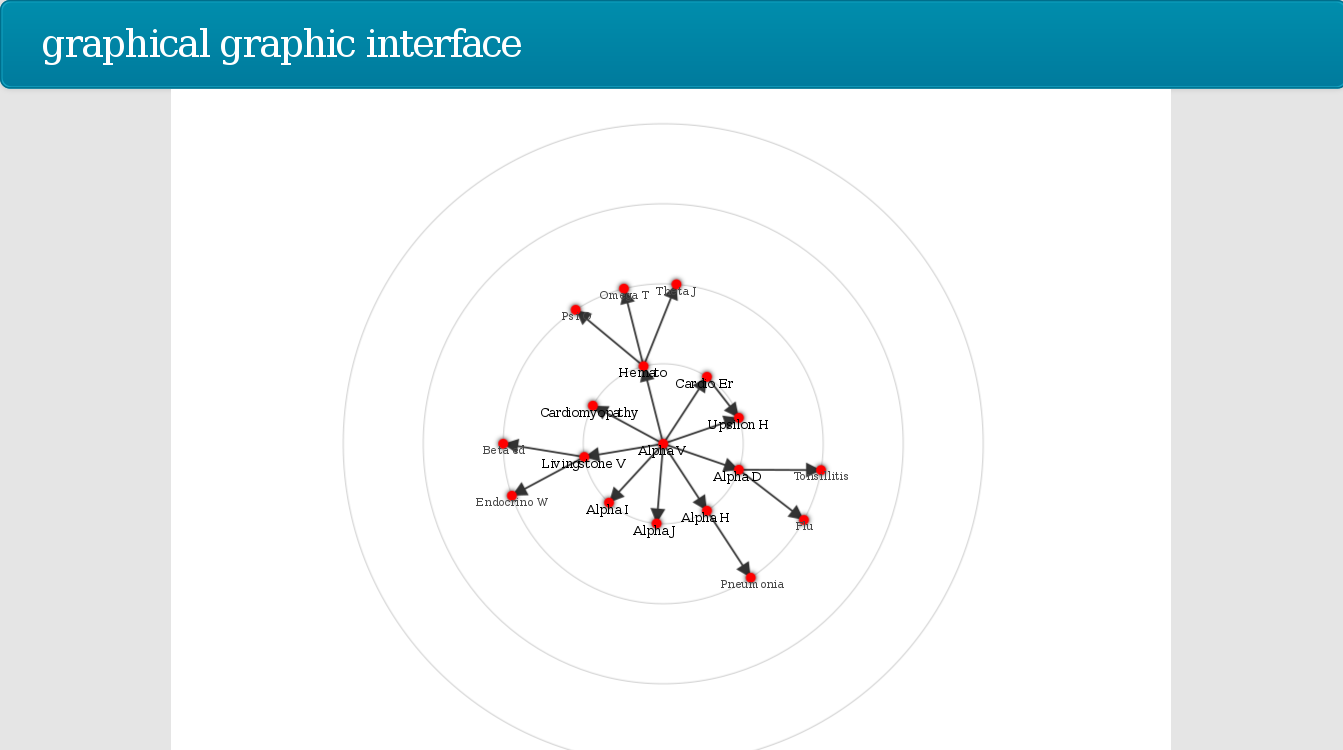
\includegraphics[scale=0.3, frame]{InterfaceGraph.png}
\caption{Node of the interest and its properties}
\end{figure}
\paragraph*{}
The user can change the node of interest by clicking on the label of the node. When the user click on the label of the node, a label appear contains the properties of the node of interest (Figure V.7).
\begin{figure}[h]
\centering
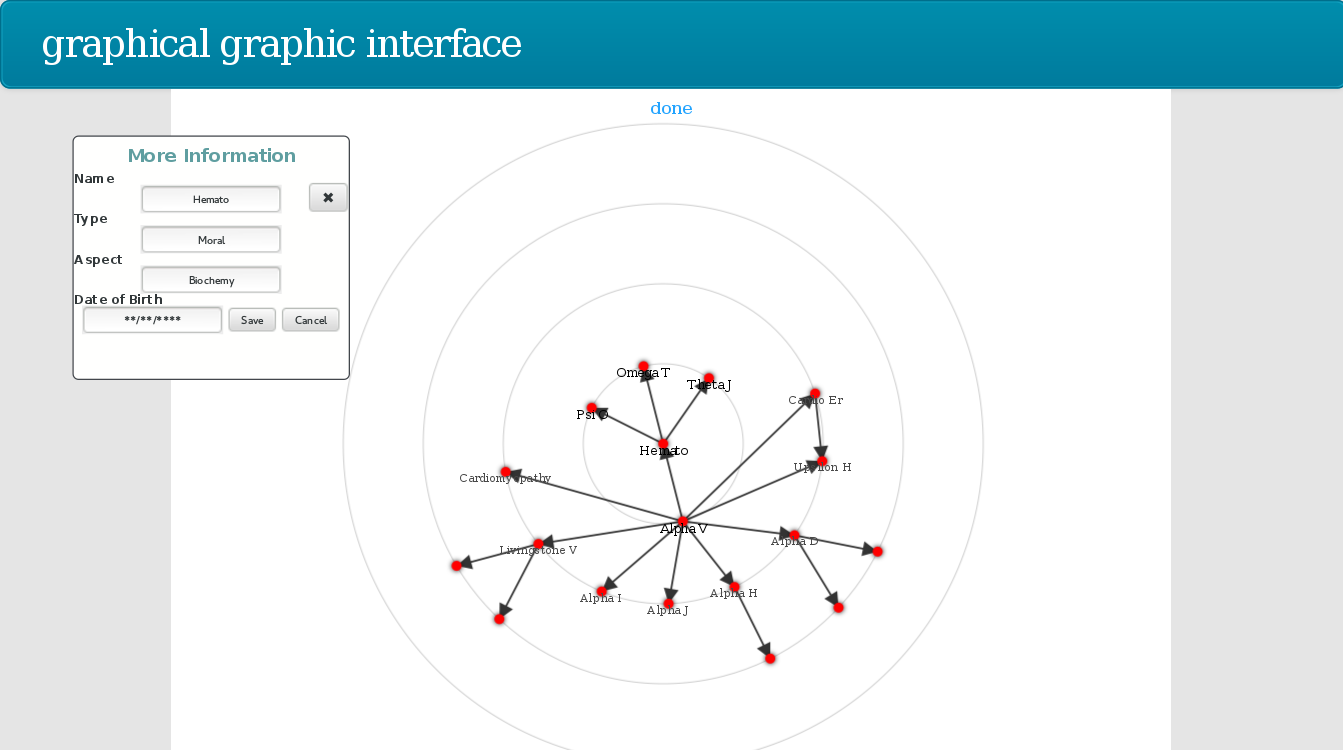
\includegraphics[scale=0.3, frame]{centericnode.png}
\caption{Interest node with her informations}
\end{figure}
\subsection{Sprint "two": managing relations and updating the nodes properties}
\paragraph*{}
In the sprint "one", only the unilateral relations have been taken into account. However, the $ IG� $ application requires relations to be unilateral, bilateral or multiple. In this sprint we implemented all the types of relations required in the specification.
We also developed a feature allowing to access to a given node properties and to add, remove or update any property.
\begin{table}[h]
\begin{center}
\begin{tabular}{|p{7cm}|p{3cm}|p{3cm}|}
\hline
\multicolumn{3}{|c|}{Sprint "two": managing relations and updating the nodes properties }  \\
\hline
\textbf{Tasks} & \textbf{Deadline} & \textbf{Date }\\
\hline
Implementation of different types of relations & 2 days & 25 April\\
\hline
Change information panel to pop-up window & 1 day & 25 April \\
\hline
Implementing the features allowing to update the properties and attributes of a given
node & 2 days & 25 April \\
\hline
\end{tabular}
\end{center}
\caption{Backlog product - Sprint "two"}
\label{Backlog product - Sprint "two"}
\end{table}
\subsubsection{Detailed design of sprint "two"}
\paragraph*{}
The Figure V.8 shows the detailed design to update node properties
\newpage
\begin{figure}[h]
\begin{center}
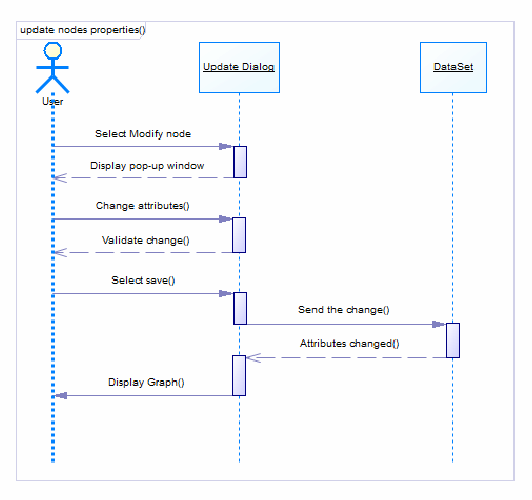
\includegraphics[scale=0.7, frame]{UpdateSEC.png}
\end{center}
\caption{Update the node properties Sequence Diagram}
\end{figure}
\subsubsection{Implementation and execution of Sprint "two"}
\paragraph*{}
The Figure V.9 presents the different types of relations. The type 1 represents unilateral/simple relation, type 2 is bilateral relation and of type 3 is multiple relation. 
\newpage
\begin{figure}[h]
\centering
\includegraphics[scale=0.4, frame]{types-of-relations.png}
\caption{types a relations handled by $IG�$}
\end{figure}
\paragraph*{}
The Figure V.10 presents the dialog, allowing users to update a given node properties.
\begin{figure}[h]
\centering
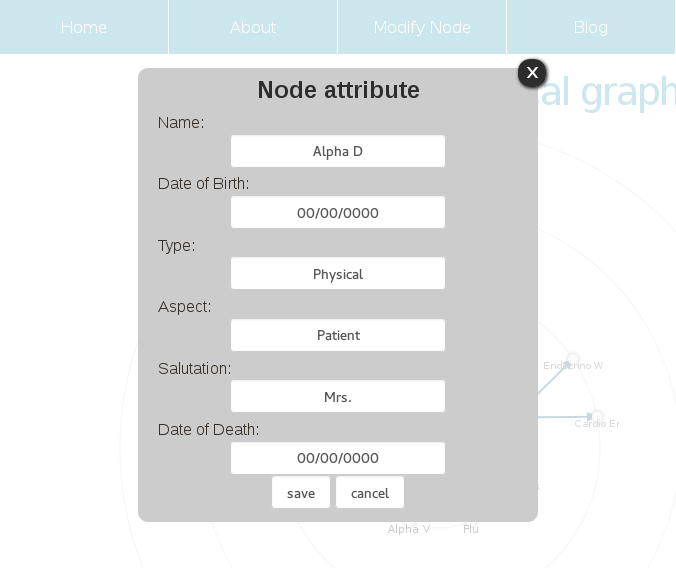
\includegraphics[scale=0.4, frame]{popupwin.png}
\caption{Updating a node}
\end{figure}
\subsection{Sprint "three": $IG�$ localization}
\paragraph*{}
The localization wasn't a requirement expressed in the specifications. During a discussion with the product owner, I noticed that the $IG�$ audience is international and I suggested to also consider the localization of the user interface in the development. The team has approved my suggestion and asked me to implement this feature in this sprint.
\begin{table}[h]
\begin{center}
\begin{tabular}{|p{7cm}|p{3cm}|p{3cm}|}
\hline
\multicolumn{3}{|c|}{Sprint3: Multilanguage and maanaging the Web application version}  \\
\hline
\textbf{Task} & \textbf{Deadline} & \textbf{Date }\\
\hline
Implementation the support of different languages & 3 days & 3 May \\
\hline
Implementing the zoom in and zoom out feature & 3 Hours & 3 May \\
\hline
Implementing Drag and Drop capablity & 3 hours & 3 May \\
\hline
Implementing the responsivity  & 2 Days & 3 May   \\
\hline
Implementing the mouseover support for edges & 2 days & 3 May\\
\hline
Manage Dropdown list for Type, Aspect and Salutation attribute & 1 hours & 3 May\\
\hline
\end{tabular}
\end{center}
\caption{Product Backlog - Sprint "three"}
\label{Product Backlog - Sprint "three"}
\end{table}
\subsubsection{Implementation and execution of Sprint "three"}
\paragraph*{}
As already mentioned  �V.7.4 the $IG�$ application is intended to be used by a wide international audience. The implementation of the software has been done in such a way that it allows the support of various locales. The user  interface language is therefore configurable. We have experimented  $IG�$ with Latin languages (French,English,Spanish,etc.), Arabic and Chinese. The Figure V.11 is a screen-shot of the English user interface of $IG�$. The Figure V.12 presents the Arabic user interface and the Chinese one is presented in the Figure  V.13
\begin{figure}[h]
\centering
\includegraphics[scale=0.4, frame]{en-lang.png}
\caption{French interface}
\end{figure}
\newpage
\paragraph*{}
\begin{figure}[h]
\centering
\includegraphics[scale=0.4, frame]{ar_lang.png}
\caption{Arabic interface}
\end{figure}
\newpage
\begin{figure}[h]
\centering
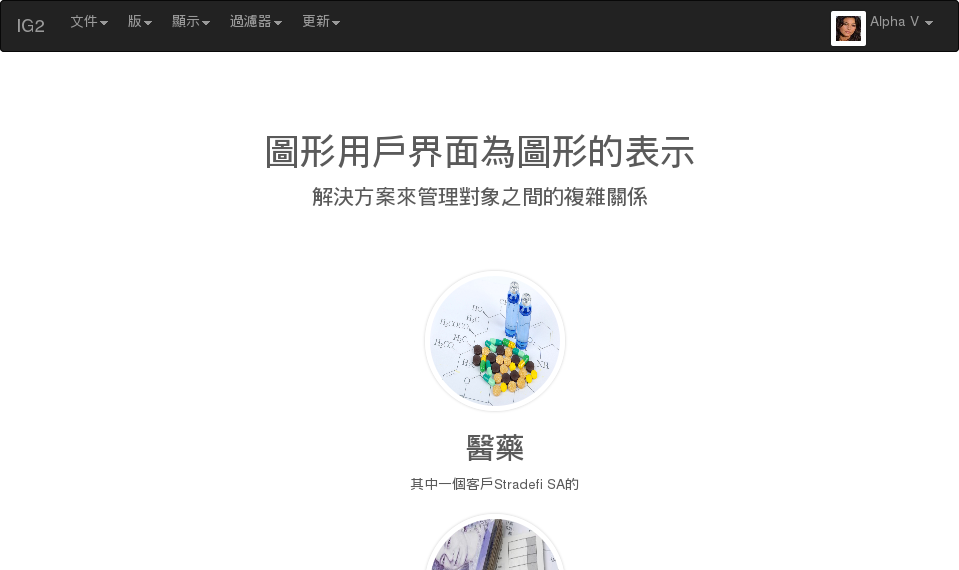
\includegraphics[scale=0.4, frame]{ch-lan.png}
\caption{Chinese interface}
\end{figure}
\paragraph*{}
The Chinese translation was done, thanks to google translator (https://translate.google.com) this translation is therefore approximate and may contain some mistakes.